\documentclass[11pt,a4paper]{article}

\usepackage[utf8]{inputenc}
\usepackage[T1]{fontenc}
\usepackage[spanish, es-nodecimaldot]{babel}
\addto\captionsspanish{\renewcommand{\tablename}{Tabla}}
\usepackage{geometry}
\geometry{margin=2.5cm}
\usepackage{booktabs}
\usepackage{array}
\usepackage{hyperref}
\hypersetup{colorlinks=true, linkcolor=black, urlcolor=blue}
\usepackage{parskip}
\usepackage{listings}
\usepackage{xcolor}
\usepackage{graphicx}
\graphicspath{{diagrams/}}
\usepackage{float}
\usepackage{caption}
\usepackage{enumitem}

\definecolor{lightgray}{gray}{0.92}
\definecolor{codered}{RGB}{180,30,30}
\definecolor{codegreen}{RGB}{0,120,0}
\definecolor{codegray}{RGB}{100,100,100}
\definecolor{warnorange}{RGB}{200,100,0}

\lstset{
  language=Java,
  basicstyle=\ttfamily\footnotesize,
  keywordstyle=\color{blue}\bfseries,
  commentstyle=\color{codegray}\itshape,
  stringstyle=\color{codegreen},
  showstringspaces=false,
  breaklines=true,
  frame=single,
  framesep=4pt,
  xleftmargin=6pt,
  xrightmargin=6pt,
  aboveskip=6pt,
  belowskip=6pt,
  numbers=left,
  numberstyle=\tiny\color{codegray},
  numbersep=5pt,
}

\newcommand{\code}[1]{\texttt{#1}}
\newcommand{\bad}[1]{\textcolor{codered}{\textbf{#1}}}
\newcommand{\good}[1]{\textcolor{codegreen}{\textbf{#1}}}
\newcommand{\warn}[1]{\textcolor{warnorange}{\textbf{#1}}}

\title{An\'alisis de la clase \code{ProbNet}\\
       \large Defectos de dise\~no, bugs y propuesta de redise\~no\\[4pt]
       \normalsize \code{org.openmarkov.core} --- paquete \code{model.network}}
\author{Manuel Arias Calleja}
\date{Marzo de 2026}

\begin{document}

\maketitle
\tableofcontents
\newpage

% ===================================================================
\section{Introducci\'on}

\code{ProbNet} es la clase m\'as cr\'itica de OpenMarkov: \textbf{490
ficheros} la referencian en todo el proyecto.  Representa una red
probabilista (bayesiana, de influencia, din\'amica, etc.) y act\'ua como
contenedor central de nodos, arcos, potenciales, restricciones y
metadatos.

Con \textbf{1440~l\'ineas} y \textbf{80+~m\'etodos p\'ublicos}, la clase
ha acumulado responsabilidades que van m\'as all\'a de su prop\'osito
original.  Este documento presenta un an\'alisis detallado de la
situaci\'on actual, identifica bugs, code smells y lagunas de testing,
y propone una hoja de ruta de redise\~no incremental.

% ===================================================================
\section{Fundamentos te\'oricos}
\label{sec:teoria}

Esta secci\'on resume los principios y patrones de ingenier\'ia del
software que se aplican ---o que se han detectado como violados--- en el
an\'alisis de \code{ProbNet}.

\subsection{Principio de Responsabilidad \'Unica (SRP)}

El \emph{Single Responsibility Principle} \cite{martin2003} establece
que \textbf{una clase debe tener una \'unica raz\'on para cambiar}.  Si
una clase acumula m\'ultiples responsabilidades, un cambio en una de
ellas puede introducir errores en las dem\'as.

\code{ProbNet} tiene al menos seis \'areas de responsabilidad distintas
(nodos, potenciales, constraints, clasificaci\'on, agentes, I/O), lo que
viola directamente este principio.

\subsection{Patr\'on \emph{Extract Class}}

\emph{Extract Class} \cite{fowler2019} es la t\'ecnica que se aplica
cuando una clase tiene demasiadas responsabilidades: se identifica un
grupo cohesivo de m\'etodos, se mueve a una nueva clase y se sustituye
en la clase original por una delegaci\'on.

En OpenMarkov, este patr\'on ya se ha aplicado con \'exito: primero con
\code{VariableTypeConverter} (extra\'ida de \code{Node}) y despu\'es con
\code{VariableStateOperations} (extra\'ida de \code{Variable}).  La
propuesta sigue el mismo precedente.

\subsection{Antipatr\'on \emph{God Class}}

Una \emph{God Class} (tambi\'en llamada \emph{Blob} o \emph{Monster
Class}) es una clase que sabe demasiado o hace demasiado
\cite{fowler2019}.  Se reconoce por:

\begin{itemize}[nosep]
  \item Cientos o miles de l\'ineas.
  \item M\'etodos que no se relacionan entre s\'i.
  \item Muchas dependencias entrantes (otros m\'odulos la necesitan para
        todo).
\end{itemize}

Con 1440~l\'ineas, 80+~m\'etodos y 490~ficheros dependientes,
\code{ProbNet} exhibe todas las caracter\'isticas de una God Class.
El objetivo del redise\~no es reducirla a su rol esencial de
\textbf{contenedor de la red probabil\'istica}, delegando las
responsabilidades secundarias.

\subsection{Principio DRY}

\emph{Don't Repeat Yourself} \cite{hunt1999} establece que cada pieza de
conocimiento debe tener una \'unica representaci\'on en el sistema.
Hemos detectado varias violaciones de DRY en \code{ProbNet}:
\code{checkProbNet()} duplica la l\'ogica de
\code{getUnsatisfiedConstraints()}, y \code{getProbPotentials()} repite
el patr\'on de \code{getUtilityPotentials()}.

\subsection{Acoplamiento}

Decimos que una clase~A est\'a \textbf{acoplada} a otra~B cuando A
necesita conocer~B para funcionar.  \code{ProbNet} almacena campos de
tipo \code{ProbNetReader} y \code{ProbNetWriter}, acoplando el modelo de
dominio al sistema de entrada/salida.  El principio de
\emph{Inversi\'on de Dependencias} (DIP) sugiere que las clases de alto
nivel (modelo) no deben depender de clases de bajo nivel (I/O).

% ===================================================================
\section{Situaci\'on actual}
\label{sec:actual}

La Figura~\ref{fig:actual} muestra un diagrama UML de \code{ProbNet}
con sus m\'etodos agrupados por responsabilidad.  Las clases asociadas
se disponen en vertical debajo de \code{ProbNet}.

\begin{figure}[H]
  \centering
  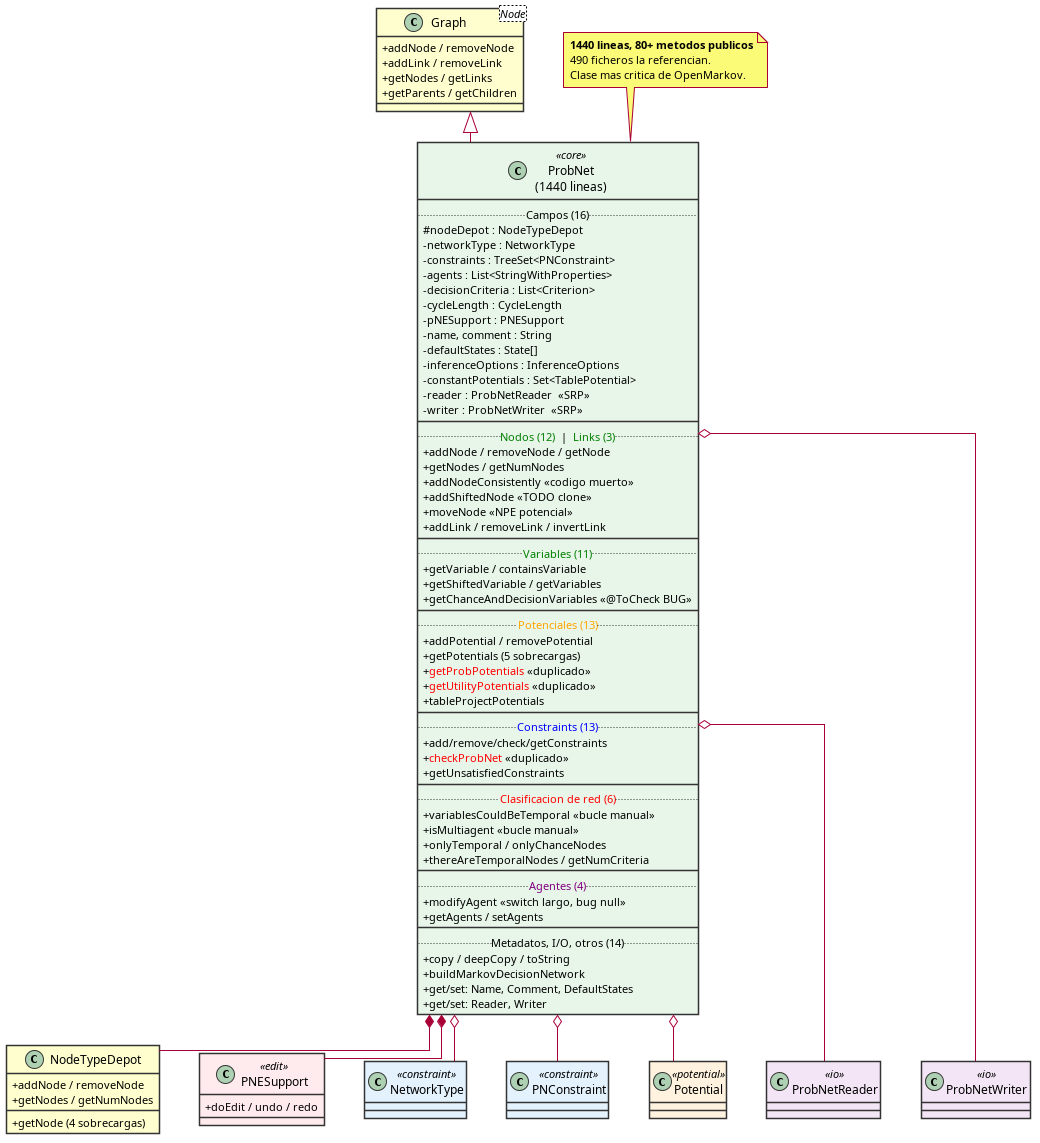
\includegraphics[width=\textwidth]{probnet-actual.png}
  \caption{Diagrama UML de \code{ProbNet} (1440~l\'ineas).  Los colores
           indican \'areas de responsabilidad; las etiquetas en rojo
           se\~nalan problemas.}
  \label{fig:actual}
\end{figure}

\code{ProbNet} extiende \code{Graph<Node>} (grafo gen\'erico) y
a\~nade:

\begin{itemize}[nosep]
  \item \textbf{16~campos}: desde \code{nodeDepot} (indexaci\'on de
        nodos por tipo) hasta \code{reader}/\code{writer} (I/O).
  \item \textbf{80+~m\'etodos p\'ublicos}: gesti\'on de nodos (12),
        links (3), variables (11), potenciales (13), constraints (13),
        clasificaci\'on de red (6), agentes (4), metadatos e I/O (12),
        y otros (copia, inferencia, criterios).
\end{itemize}

% ===================================================================
\section{Bugs detectados}
\label{sec:bugs}

La Figura~\ref{fig:bugs} resume los bugs, code smells y riesgos de tipo
identificados.

\begin{figure}[H]
  \centering
  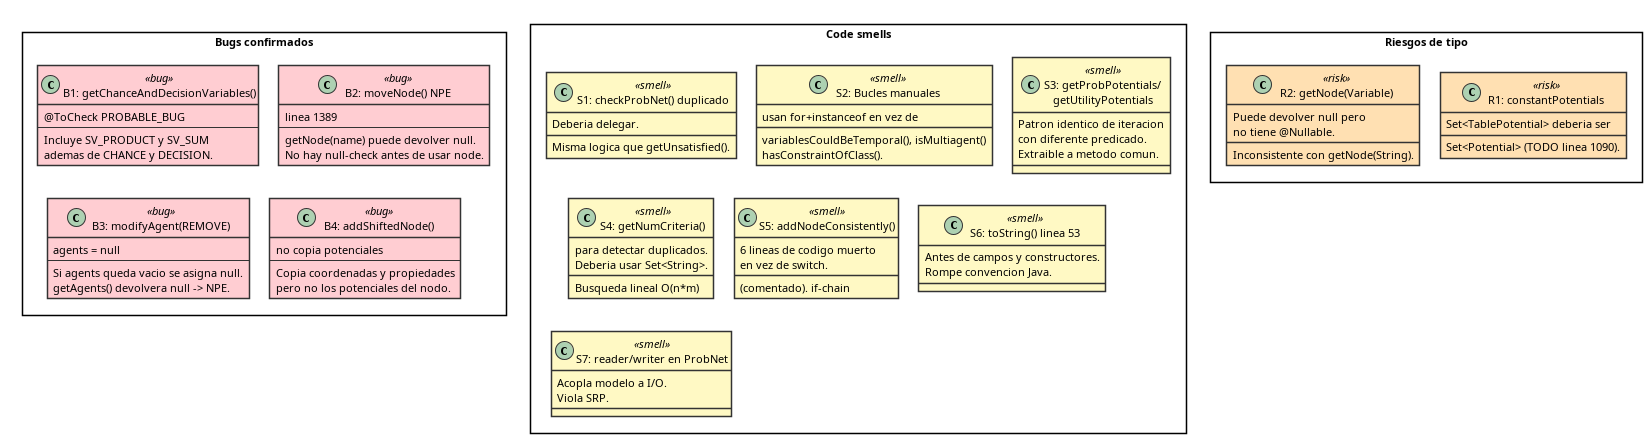
\includegraphics[width=\textwidth]{bugs-detectados.png}
  \caption{Bugs confirmados (rojo), code smells (amarillo) y riesgos
           de tipo (naranja) detectados en \code{ProbNet}.}
  \label{fig:bugs}
\end{figure}

\subsection{B1: \code{getChanceAndDecisionVariables()} incluye tipos extra}

El m\'etodo est\'a anotado con \code{@ToCheck(PROBABLE\_BUG)}.  Su
nombre indica que devuelve solo variables de tipo CHANCE y DECISION,
pero el \code{switch} tambi\'en incluye \code{SV\_PRODUCT} y
\code{SV\_SUM}:

\begin{lstlisting}
case CHANCE, SV_PRODUCT, SV_SUM, DECISION -> true;
case UTILITY -> false;
\end{lstlisting}

Si el comportamiento actual es intencionado, el nombre del m\'etodo es
enga\~noso.  Si no lo es, devuelve variables de m\'as.

\subsection{B2: \code{moveNode()} --- NullPointerException potencial}

En la l\'inea~1389, \code{getNode(name)} puede devolver \code{null}
si el nombre no existe en la red.  No hay comprobaci\'on de nulidad
antes de llamar a \code{node.setCoordinateX()}.

\begin{lstlisting}
Node node = getNode(name);
node.setCoordinateX(newPositions.get(i).getX()); // NPE si node == null
\end{lstlisting}

\subsection{B3: \code{modifyAgent(REMOVE)} deja \code{agents = null}}

Cuando se elimina el \'ultimo agente, el m\'etodo asigna
\code{agents = null} (l\'inea~1426).  Sin embargo, \code{getAgents()}
devuelve directamente el campo sin comprobaci\'on, lo que causa un
\code{NullPointerException} en cualquier c\'odigo que itere sobre el
resultado.  Adem\'as, \code{modifyAgent(ADD)} crea la lista si es
\code{null}, pero nunca deber\'ia haberlo sido.

\subsection{B4: \code{addShiftedNode()} no copia potenciales}

El m\'etodo copia el tipo de nodo, coordenadas, prop\'osito, relevancia,
comentario y propiedades adicionales, pero \textbf{no copia los
potenciales} del nodo original ni crea uno por defecto.  El propio
c\'odigo reconoce el problema:

\begin{lstlisting}
// TODO Hacer clon para node y quitar estas lineas
\end{lstlisting}

% ===================================================================
\section{Code smells}
\label{sec:smells}

\subsection{S1: L\'ogica duplicada en \code{checkProbNet()} y
            \code{getUnsatisfiedConstraints()} (violaci\'on DRY)}

Ambos m\'etodos iteran sobre \code{constraints} con la misma condici\'on
\code{constraint.isMetBy(this)}.  La soluci\'on trivial:

\begin{lstlisting}
public boolean checkProbNet() {
    return getUnsatisfiedConstraints().isEmpty();
}
\end{lstlisting}

\subsection{S2: Bucles manuales en clasificaci\'on de red}

\code{variablesCouldBeTemporal()} e \code{isMultiagent()} usan un bucle
\code{for} manual sobre \code{constraints} con \code{instanceof},
cuando ya existe \code{hasConstraintOfClass()} que hace exactamente
eso:

\begin{lstlisting}
// Antes (7 lineas):
public boolean variablesCouldBeTemporal() {
    for (PNConstraint constraint : constraints) {
        if (constraint instanceof OnlyAtemporalVariables) return false;
    }
    return true;
}

// Despues (1 linea):
public boolean variablesCouldBeTemporal() {
    return !hasConstraintOfClass(OnlyAtemporalVariables.class);
}
\end{lstlisting}

\subsection{S3: Patr\'on duplicado en
            \code{getProbPotentials()}/\code{getUtilityPotentials()} (violaci\'on DRY)}

Ambos m\'etodos siguen el mismo patr\'on: obtener el nodo de la
variable, recopilar vecinos, iterar potenciales y filtrar.  Solo
difiere el predicado de filtro.  Se podr\'ian unificar en un m\'etodo
privado parametrizado o extraer a una clase de consultas.

\subsection{S4: \code{getNumCriteria()} con complejidad $O(n \cdot m)$}

Usa una \code{List<String>} y b\'usqueda lineal para detectar duplicados
en lugar de un \code{Set<String>}, resultando en complejidad
cuadr\'atica innecesaria.

\subsection{S5: C\'odigo comentado en \code{addNodeConsistently()}}

Las l\'ineas 933--938 contienen 6~l\'ineas de c\'odigo comentado que
nunca se ejecutan.  Adem\'as, usa una cadena de \code{if} en lugar de
\code{switch}.

\subsection{S6: \code{toString()} en la l\'inea~53}

El m\'etodo \code{toString()} est\'a al inicio del fichero, antes
incluso de la declaraci\'on de campos.  Rompe la estructura convencional
de Java (campos $\to$ constructores $\to$ m\'etodos).

\subsection{S7: \code{reader}/\code{writer} almacenados en ProbNet
            (violaci\'on SRP y DIP)}

\code{ProbNet} almacena referencias a \code{ProbNetReader} y
\code{ProbNetWriter}, acoplando el modelo de dominio al sistema de
I/O.  El reader/writer solo se usa en la GUI para recordar qu\'e formato
se us\'o.  Esta informaci\'on deber\'ia residir en el controlador de
ficheros, no en el modelo de dominio.

% ===================================================================
\section{Cobertura de tests}
\label{sec:tests}

Las siguientes figuras muestran el estado de la cobertura de tests por
\'area funcional.  El c\'odigo de colores: \good{verde} = testado,
\warn{amarillo} = parcialmente testado, \bad{rojo} = sin tests.

\subsection{Nodos, links y variables}

\begin{figure}[H]
  \centering
  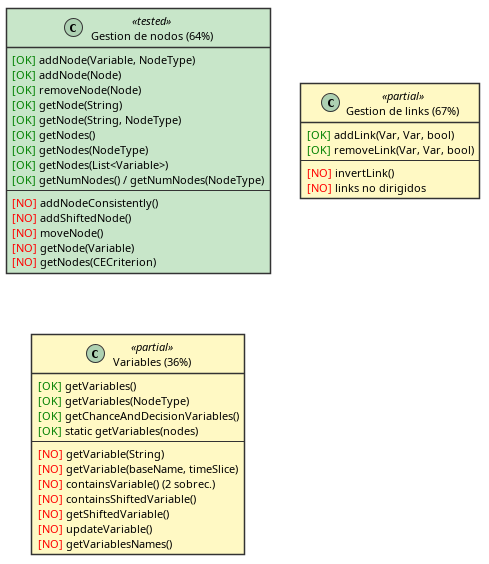
\includegraphics[width=\textwidth]{cobertura-nodos-links-vars.png}
  \caption{Cobertura de tests: nodos (64\%), links (67\%) y variables
           (36\%).}
  \label{fig:cob-nlv}
\end{figure}

\subsection{Potenciales, constraints y copia}

\begin{figure}[H]
  \centering
  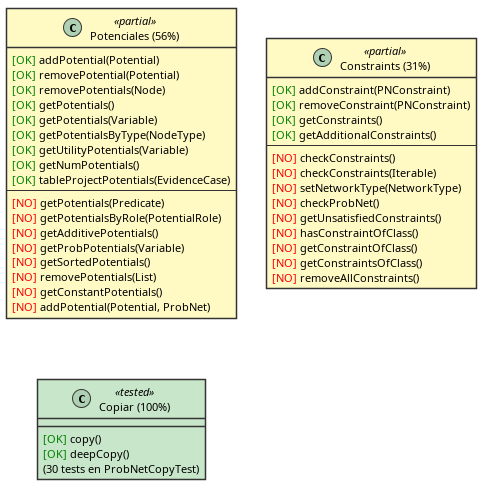
\includegraphics[width=\textwidth]{cobertura-potenciales-constraints.png}
  \caption{Cobertura de tests: potenciales (56\%), constraints (31\%)
           y copia (100\%).}
  \label{fig:cob-pc}
\end{figure}

\subsection{Clasificaci\'on, agentes e I/O}

\begin{figure}[H]
  \centering
  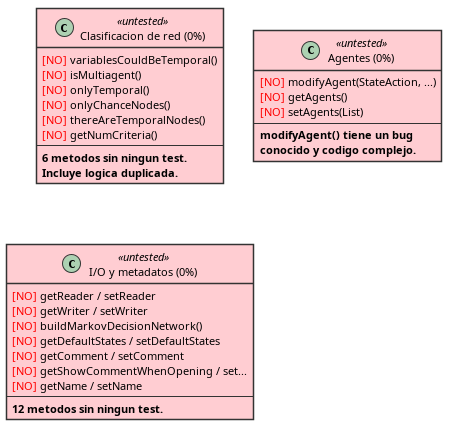
\includegraphics[width=\textwidth]{cobertura-clasificacion-agentes-io.png}
  \caption{Cobertura de tests: clasificaci\'on de red (0\%), agentes
           (0\%) e I/O y metadatos (0\%).  Estas tres \'areas son las
           lagunas m\'as cr\'iticas.}
  \label{fig:cob-cai}
\end{figure}

\subsection{Resumen cuantitativo}

\begin{center}
\begin{tabular}{lccr}
\toprule
\textbf{\'Area} & \textbf{M\'etodos} & \textbf{Testados} & \textbf{Cobertura} \\
\midrule
Gesti\'on de nodos        & 14 & 9  & 64\% \\
Gesti\'on de links        & 3  & 2  & 67\% \\
Variables                  & 11 & 4  & 36\% \\
Potenciales                & 16 & 9  & 56\% \\
Constraints                & 13 & 4  & 31\% \\
Clasificaci\'on de red     & 6  & 0  & \bad{0\%} \\
Agentes                    & 4  & 0  & \bad{0\%} \\
Copiar                     & 2  & 2  & 100\% \\
I/O y metadatos            & 12 & 0  & \bad{0\%} \\
\midrule
\textbf{Total}             & \textbf{81} & \textbf{30} & \textbf{37\%} \\
\bottomrule
\end{tabular}
\end{center}

Existen \textbf{30~tests} en \code{ProbNetTest} y \textbf{30~tests} en
\code{ProbNetCopyTest}, pero \textbf{51~m\'etodos p\'ublicos} no tienen
ning\'un test unitario directo.

% ===================================================================
\section{Propuesta de redise\~no}
\label{sec:propuesta}

Dado que \code{ProbNet} es referenciada por 490~ficheros, toda
refactorizaci\'on debe ser \textbf{incremental} y
\textbf{retrocompatible}.  Se aplica el patr\'on \emph{Extract Class}
siguiendo el precedente de \code{VariableTypeConverter} y
\code{VariableStateOperations}.

La Figura~\ref{fig:propuesta} muestra la arquitectura objetivo.

\begin{figure}[H]
  \centering
  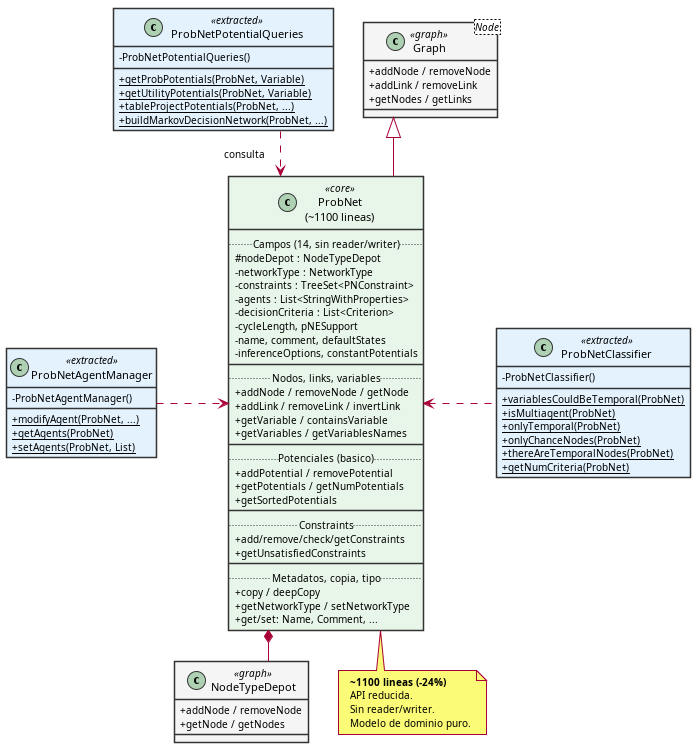
\includegraphics[width=\textwidth]{probnet-propuesta.png}
  \caption{Arquitectura propuesta: \code{ProbNet} reducida a
           $\sim$1100~l\'ineas, con tres clases de utilidad est\'atica
           extra\'idas.}
  \label{fig:propuesta}
\end{figure}

\subsection{Fase 0: Ampliar tests (prerrequisito)}

Antes de cualquier refactorizaci\'on, cubrir las lagunas cr\'iticas:

\begin{center}
\footnotesize
\begin{tabular}{lp{8cm}r}
\toprule
\textbf{\'Area} & \textbf{Tests a a\~nadir} & \textbf{Prioridad} \\
\midrule
Variables & \code{getVariable}, \code{containsVariable},
            \code{getShiftedVariable}, \code{getVariablesNames},
            \code{updateVariable} & Alta \\
Constraints & \code{setNetworkType} (cambio v\'alido e inv\'alido con
              rollback), \code{checkProbNet},
              \code{getUnsatisfiedConstraints},
              \code{hasConstraintOfClass} & Alta \\
Clasificaci\'on & Todos los 6~m\'etodos con redes BN, ID y DBN & Alta \\
Agentes & \code{modifyAgent} ADD/REMOVE/RENAME con casos l\'imite & Alta \\
Potenciales & \code{addPotential(pot, origNet)},
              \code{getProbPotentials}, \code{getSortedPotentials},
              \code{getConstantPotentials} & Media \\
Nodos & \code{moveNode} (caso normal y nombre inv\'alido),
        \code{addShiftedNode}, \code{invertLink} & Media \\
Metadatos & \code{getDefaultStates}, \code{comment},
            \code{showCommentWhenOpening} & Baja \\
\bottomrule
\end{tabular}
\end{center}

Objetivo: pasar de \textbf{37\%} a \textbf{$>$80\%} de cobertura de
m\'etodos p\'ublicos antes de empezar las extracciones.

\subsection{Fase 1: Corregir bugs (sin cambio de API)}

\begin{center}
\begin{tabular}{lp{9cm}}
\toprule
\textbf{Bug} & \textbf{Correcci\'on propuesta} \\
\midrule
B1 & Renombrar a \code{getNonUtilityVariables()} o eliminar
     \code{SV\_PRODUCT}/\code{SV\_SUM} del switch seg\'un la intenci\'on
     original (requiere consultar el uso en el proyecto). \\
B2 & A\~nadir null-check en \code{moveNode()} con
     \code{Objects.requireNonNull} o skip silencioso. \\
B3 & Inicializar \code{agents} como lista vac\'ia en lugar de
     \code{null}; eliminar asignaci\'on \code{agents = null} en
     \code{modifyAgent(REMOVE)}. \\
B4 & En \code{addShiftedNode()}, a\~nadir copia de potenciales o crear
     potencial uniforme por defecto (verificar qu\'e espera el
     c\'odigo llamador). \\
\bottomrule
\end{tabular}
\end{center}

\subsection{Fase 2: Simplificaciones internas (sin cambio de API)}

\begin{enumerate}
  \item \code{checkProbNet()} $\to$ delegar en
        \code{getUnsatisfiedConstraints().isEmpty()} (eliminar
        duplicaci\'on DRY).
  \item \code{variablesCouldBeTemporal()} e \code{isMultiagent()} $\to$
        usar \code{hasConstraintOfClass()} (eliminar bucles manuales).
  \item \code{getNumCriteria()} $\to$ usar \code{Set<String>} (mejorar
        complejidad algor\'itmica).
  \item Eliminar c\'odigo comentado en \code{addNodeConsistently()},
        convertir if-chain a switch.
  \item Mover \code{toString()} despu\'es de los campos.
  \item A\~nadir \code{@Nullable} a \code{getNode(Variable)}.
\end{enumerate}

\subsection{Fase 3: Extraer \code{ProbNetClassifier} (\emph{Extract Class})}

Mover los 6~m\'etodos de clasificaci\'on de red
(\code{variablesCouldBeTemporal}, \code{isMultiagent},
\code{onlyTemporal}, \code{onlyChanceNodes},
\code{thereAreTemporalNodes}, \code{getNumCriteria}) a una clase de
utilidad est\'atica.  Dejar delegaciones en \code{ProbNet} para
retrocompatibilidad.

\subsection{Fase 4: Extraer \code{ProbNetAgentManager} (\emph{Extract Class})}

Mover \code{modifyAgent()}, \code{getAgents()}, \code{setAgents()} a
una clase separada.  La l\'ogica de agentes es completamente
independiente del resto de \code{ProbNet} y solo se usa desde la GUI.

\subsection{Fase 5: Extraer \code{ProbNetPotentialQueries} (\emph{Extract Class})}

Mover \code{getProbPotentials()}, \code{getUtilityPotentials()},
\code{tableProjectPotentials()} y \code{buildMarkovDecisionNetwork()} a
una clase de consultas.  Unificar los patrones duplicados de iteraci\'on
sobre vecinos (eliminando la violaci\'on DRY).

\subsection{Fase 6: Evaluar extracci\'on de reader/writer (reducir acoplamiento)}

Evaluar mover \code{reader}/\code{writer} fuera de \code{ProbNet} hacia
el controlador de ficheros de la GUI.  Esto reducir\'ia el acoplamiento
del modelo con el sistema de I/O (DIP).  Requiere un an\'alisis de
impacto en los m\'odulos \code{gui} e \code{io}.

% ===================================================================
\section{Resumen de impacto estimado}

\begin{center}
\begin{tabular}{lrr}
\toprule
\textbf{M\'etrica} & \textbf{Actual} & \textbf{Objetivo} \\
\midrule
L\'ineas de \code{ProbNet.java}        & 1440  & $\sim$1100 \\
M\'etodos p\'ublicos en \code{ProbNet} & 80+   & $\sim$65 \\
Bugs conocidos                          & 4     & 0 \\
Code smells                             & 7     & 0 \\
Cobertura de tests                      & 37\%  & $>$80\% \\
Clases de utilidad nuevas               & 0     & 3 \\
\bottomrule
\end{tabular}
\end{center}

% ===================================================================
\section{Orden de ejecuci\'on y riesgos}

\begin{center}
\begin{tabular}{clcc}
\toprule
\textbf{Fase} & \textbf{Descripci\'on} & \textbf{Riesgo} & \textbf{Dependencia} \\
\midrule
0 & Ampliar tests          & Bajo  & --- \\
1 & Corregir bugs          & Bajo  & Fase~0 \\
2 & Simplificaciones       & Bajo  & Fase~0 \\
3 & Extraer Classifier     & Medio & Fase~0, 2 \\
4 & Extraer AgentManager   & Bajo  & Fase~0, 1 \\
5 & Extraer PotentialQueries & Medio & Fase~0 \\
6 & Evaluar reader/writer  & Alto  & Fase~0 \\
\bottomrule
\end{tabular}
\end{center}

Las fases 0--2 son de bajo riesgo y alto valor.  Las fases 3--5 siguen
el patr\'on \emph{Extract Class} ya probado con \'exito en
\code{VariableStateOperations} y \code{VariableTypeConverter}.  La
fase~6 requiere un an\'alisis adicional del m\'odulo GUI.

\textbf{Principio rector}: cada fase debe dejar todos los tests pasando
y no romper la API p\'ublica existente.  Los m\'etodos extra\'idos se
delegan desde \code{ProbNet} hasta que los llamadores puedan migrar.

% ===================================================================
\begin{thebibliography}{9}

\bibitem{fowler2019}
  M. Fowler,
  \emph{Refactoring: Improving the Design of Existing Code},
  2nd ed., Addison-Wesley, 2019.

\bibitem{martin2003}
  R.C. Martin,
  \emph{Agile Software Development: Principles, Patterns, and Practices},
  Prentice Hall, 2003.

\bibitem{hunt1999}
  A. Hunt, D. Thomas,
  \emph{The Pragmatic Programmer},
  Addison-Wesley, 1999.

\end{thebibliography}

\end{document}
